
\section{Validation set approach}
\subsection{Theory}
The Validation set approach works by splitting the data to two parts one is called the training set and the other is called the testing set(validation or hold-out set). An example of the split can be seen on Figure \ref{fig:validationsetapproach}. The model is trained with the training set, after the training is finished the model is tested with the testing set, which the model was not trained on. This test produces a test error, in the form of MSE, which is good for validating the model. The advantage of this method is low computation time, but the results of this method is depended on which data points will end up in the sets. 
\begin{figure}[H]
	\centering
	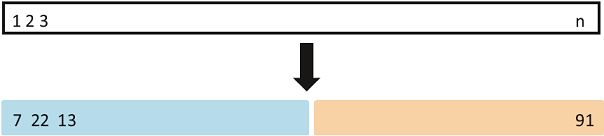
\includegraphics[width=0.4\linewidth]{crossValidation/validationSetApproach}
	\caption{Validation set approach. The entire dataset is split randomly into a training and testing set.}
	\label{fig:validationsetapproach}
\end{figure}

\subsection{Result}
\subsubsection*{LAB 5.3.1}%TODO write full lab
In lab 5.3.1 the validation set approach is used to find estimate the test error that result from fitting linear models on the Auto data\footnote{https://raw.github.com/vincentarelbundock/Rdatasets/master/csv/ISLR/Auto.csv} set. First thing is to split the Auto dataset into a training by taking 196 random samples out of the data and use the rest for the testing. We train the model and get the following MSE
\begin{lstlisting}
23.36190289258723
\end{lstlisting}
The MSE looks high so a way to reduce the MSE could be with a polynomial 
\begin{lstlisting}[language=Python]
--------Test Error for 2nd order--------
20.25269085835005
\end{lstlisting}
Cubic regression.
\begin{lstlisting}[language=Python]
--------Test Error for 3rd order--------
20.325609365773605
\end{lstlisting}
By reviewing the results it is clear that the MSE for the models with linear, quadratic, and cubic terms are 23.36, 20.25, and 20.33.

